\documentclass{standalone}
%<--------------------------------------------------------------------------->%
%%% Math %%%
\usepackage{amsmath,amssymb}
\usepackage{mathrsfs,gensymb}
\usepackage{mathtools}
% \usepackage{centernot}
% \usepackage{accents}
% \usepackage[makeroom]{cancel}
% \newcommand{\two}[2]{\substack{ \text{#1} \\ \text{#2} }}
% \newcommand{\raum}{\phantom{=}{\:\,}}
% \newcommand{\st}{s.t.\ }
% \newcommand{\asDemonstrated}{\null\nobreak\hfill\ensuremath{\blacksquare}}
%-----------------------------------------------------------------------------%
%%% TikZ %%%
\usepackage{tikz}
\usetikzlibrary{calc}
% \usetikzlibrary{angles,quotes}
% \usetikzlibrary{intersections,topaths}
% \usetikzlibrary{decorations.markings}
%<--------------------------------------------------------------------------->%

\begin{document}

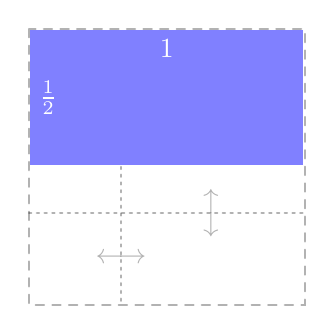
\begin{tikzpicture}[scale=3.5,thick,line cap=round,yscale=-1]
	\tikzstyle{jiao}=[solid,circle,draw,fill=white,inner sep=.8pt];
	\tikzstyle{tile1}=[line width=0.1em,draw=white,fill=blue!50];
\tikzstyle{tile2}=[line width=0.1em,draw=white,fill=red!50];
\tikzstyle{tile3}=[line width=0.1em,draw=white,fill=blue!50!red!60];
\tikzstyle{tile4}=[line width=0.1em,draw=white,fill=blue!20!red!60];

	\draw[tile1] (0,0) rectangle (1,1/2);
	\draw[dashed,draw,opacity=0.3] (0,0) rectangle (1,1);
	\draw[dotted,draw,opacity=0.3] (1/3,1/2) -- node[pos=2/3]{$\longleftrightarrow$} +(0,1/2);
	\draw[dotted,draw,opacity=0.3] (0,2/3) -- node[rotate=90,pos=2/3]{$\longleftrightarrow$} +(1,0);
	\node[white,below] at (1/2,0) {1};
	\node[white,right] at (0,1/4) {$\frac12$};
\end{tikzpicture}

\end{document}
